The client will need to stay updated with the current contents of the 
spreadsheet, so this protocol provides an \hyperref[sec:message:open]{open} 
command, which will accept the \emph{id} of the spreadsheet that the client 
would like to open. The server will respond to this command with the current 
contents of the spreadsheet, as well as adding the client as a subscriber to 
all future \hyperref[sec:message:updates]{updates} regarding the spreadsheets. These updates will contain the 
current state of the spreadsheet and delete and rename notifications for the 
spreadsheet. 

\begin{figure}[H]
    \begin{center}
        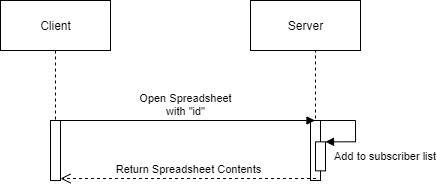
\includegraphics[width=2.5in]{Figures/open_sprd.png}
        \caption{Opening a spreadsheet sequence}
    \end{center}
\end{figure}